\documentclass{article}

\usepackage{graphicx}
\usepackage[utf8]{inputenc}
\usepackage[english]{babel}
\usepackage[document]{ragged2e}



\begin{document}

\textbf{Q2}  
\textbf{ Image Segmentation using Mean Shift}
\vskip 0.2in

Pranav Sankhe \texttt{150070009} \newline
Kalpesh Krishna \texttt{140070017}  \newline
Mohit Madan \texttt{15D070028} \newline

\vskip 0.5in

\textbf{Report:}  
\vskip 0.1in



\begin{figure}[h!]
  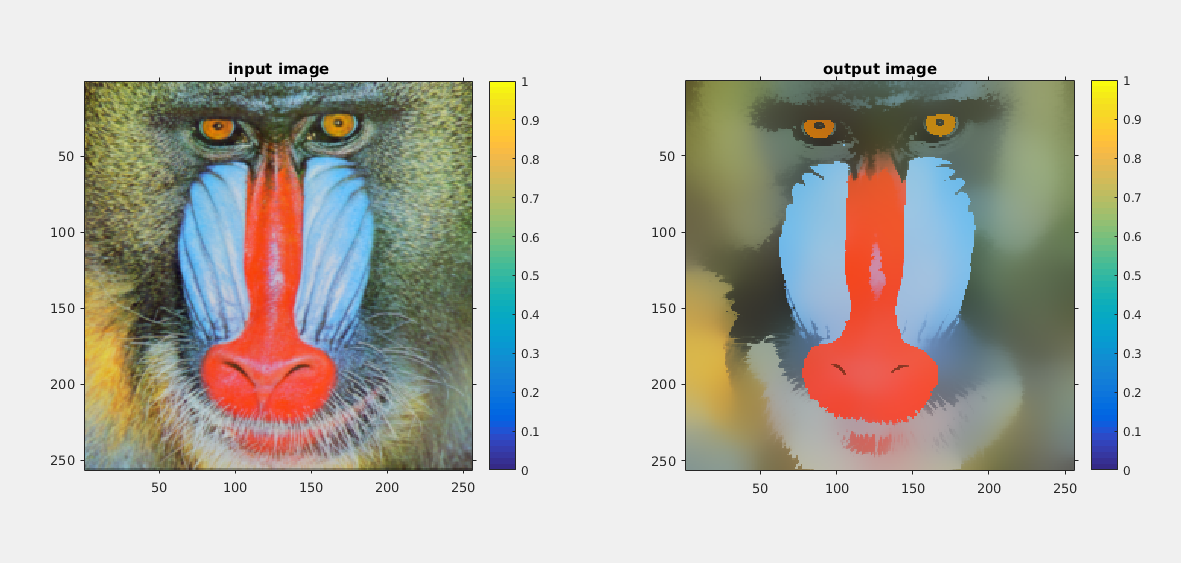
\includegraphics[width=\linewidth]{without_bin.png}
  \caption{Original image along with the segmented image that shows color-coded pixels using the color component of the converged feature vectors.}
  \label{fig:result1}
\end{figure}


\begin{figure}[h!]
  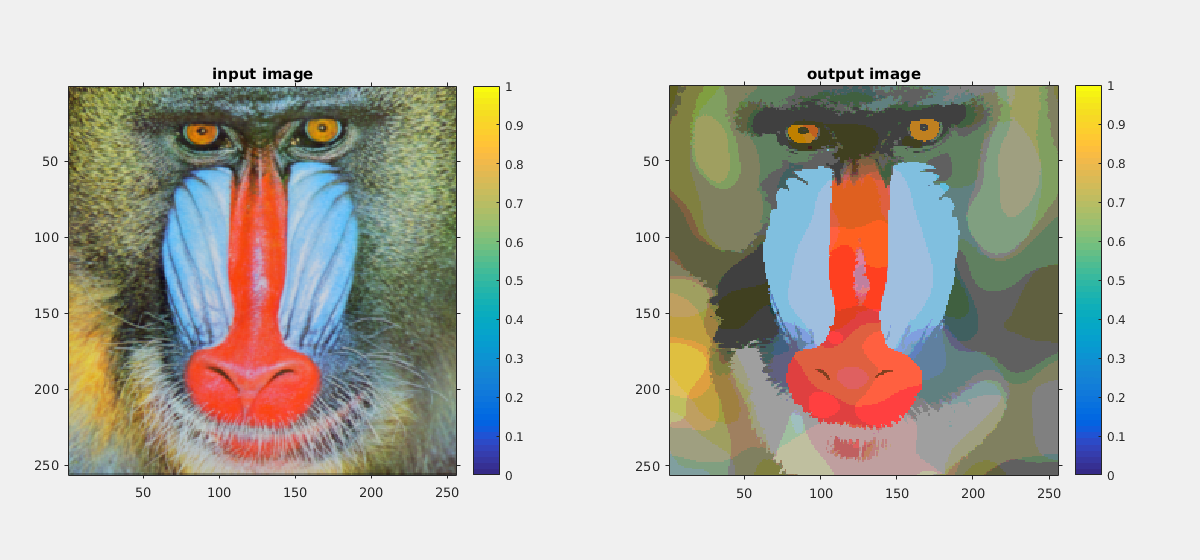
\includegraphics[width=\linewidth]{with_bin.png}
  \caption{Result after bining}
  \label{fig:result2}
\end{figure}

\newpage

\textbf{Kernel bandwidth for the color feature} \texttt{= 0.1} \newline
\textbf{Gaussian kernel bandwidth for the spatial feature} \texttt{= 10} \newline
\textbf{Number of Iterations} \texttt{= 15} \newline


\end{document}